\documentclass{exam}
\usepackage{tikz}
\usepackage{amssymb}
\usepackage{amsmath}
\title{CS113/DISCRETE MATHEMATICS-SPRING 2024}
\author{Worksheet 25}
\date{Topic: Paths, Circuits, Graph Connectivity }
\begin{document}
\maketitle
\vspace{5mm}
\begin{center}
\fbox{\fbox{\parbox{5.5in}{\centering Today, we're once again diving into the  world of graphs, exploring two fundamental concepts: paths and connectivity. These ideas are at the core of graph theory, from planning efficient routes to analyzing communication networks, understanding paths and connectivity empowers us to make smart decisions. Happy Learning!}}}
\end{center}
\vspace{5mm}

\makebox[0.75\textwidth]{Student's Name and ID:\enspace\hrulefill} 

\vspace{5mm}
\makebox[0.75\textwidth]{Instructor’s name:\enspace\hrulefill}

\vspace{10mm}





\begin{questions}

\question
Use paths either to show that these graphs are not isomorphic or to find an isomorphism between these graphs.

\vspace{1in}
\begin{parts}
\part
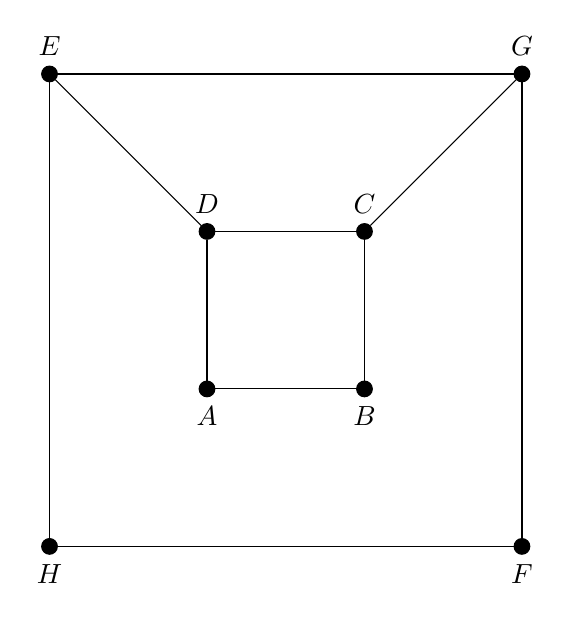
\begin{tikzpicture}
\node[circle, draw, fill, inner sep=2pt, label=below:$A$] (A) at (0,0) {};
\node[circle, draw, fill, inner sep=2pt, label=below:$B$] (B) at (2,0) {};
\node[circle, draw, fill, inner sep=2pt, label=above:$C$] (C) at (2,2) {};
\node[circle, draw, fill, inner sep=2pt, label=above:$D$] (D) at (0,2) {};
\node[circle, draw, fill, inner sep=2pt, label=above:$E$] (E) at (-2,4) {};
\node[circle, draw, fill, inner sep=2pt, label=below:$F$] (F) at (4,-2) {};
\node[circle, draw, fill, inner sep=2pt, label=above:$G$] (G) at (4,4) {};
\node[circle, draw, fill, inner sep=2pt, label=below:$H$] (H) at (-2,-2) {};


\draw (A) -- (B) -- (C) -- (D) -- (A);
\draw (E) -- (H) -- (F) -- (G) -- (E);
\draw (E)--(D);
\draw (C)--(G);

\end{tikzpicture}

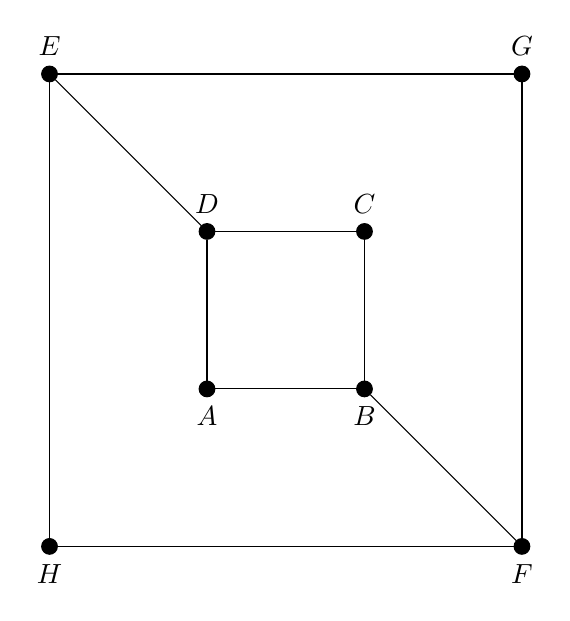
\begin{tikzpicture}
\node[circle, draw, fill, inner sep=2pt, label=below:$A$] (A) at (0,0) {};
\node[circle, draw, fill, inner sep=2pt, label=below:$B$] (B) at (2,0) {};
\node[circle, draw, fill, inner sep=2pt, label=above:$C$] (C) at (2,2) {};
\node[circle, draw, fill, inner sep=2pt, label=above:$D$] (D) at (0,2) {};
\node[circle, draw, fill, inner sep=2pt, label=above:$E$] (E) at (-2,4) {};
\node[circle, draw, fill, inner sep=2pt, label=below:$F$] (F) at (4,-2) {};
\node[circle, draw, fill, inner sep=2pt, label=above:$G$] (G) at (4,4) {};
\node[circle, draw, fill, inner sep=2pt, label=below:$H$] (H) at (-2,-2) {};


\draw (A) -- (B) -- (C) -- (D) -- (A);
\draw (E) -- (H) -- (F) -- (G) -- (E);
\draw (E) -- (D);
\draw (B) --(F);
\end{tikzpicture}
\newpage

\part
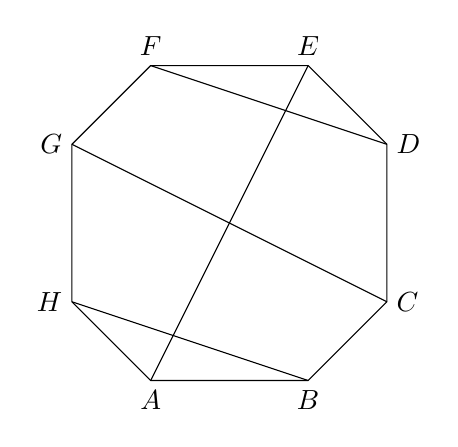
\begin{tikzpicture}
  % Define the coordinates for the octagon vertices
  \coordinate[label=below:$A$] (A) at (0,0);
  \coordinate[label=below:$B$] (B) at (2,0);
  \coordinate[label=right:$C$] (C) at (3,1);
  \coordinate[label=right:$D$] (D) at (3,3);
  \coordinate[label=above:$E$] (E) at (2,4);
  \coordinate[label=above:$F$] (F) at (0,4);
  \coordinate[label=left:$G$] (G) at (-1,3);
  \coordinate[label=left:$H$] (H) at (-1,1);
  
  % Draw the octagon
  \draw (A) -- (B) -- (C) -- (D) -- (E) -- (F) -- (G) -- (H) -- cycle;
  \draw (F) --(D);
  \draw (G)--(C);
  \draw (H)--(B);
  \draw (E)--(A);
\end{tikzpicture}

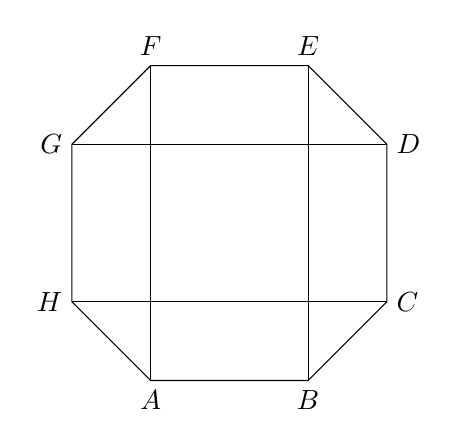
\begin{tikzpicture}
  % Define the coordinates for the octagon vertices
  \coordinate[label=below:$A$] (A) at (0,0);
  \coordinate[label=below:$B$] (B) at (2,0);
  \coordinate[label=right:$C$] (C) at (3,1);
  \coordinate[label=right:$D$] (D) at (3,3);
  \coordinate[label=above:$E$] (E) at (2,4);
  \coordinate[label=above:$F$] (F) at (0,4);
  \coordinate[label=left:$G$] (G) at (-1,3);
  \coordinate[label=left:$H$] (H) at (-1,1);
  
  % Draw the octagon
  \draw (A) -- (B) -- (C) -- (D) -- (E) -- (F) -- (G) -- (H) -- cycle;
  \draw(F)--(A);
  \draw(E)--(B);
  \draw(H)--(C);
  \draw(G)--(D);
  
\end{tikzpicture}
\newpage
\end{parts}

\question
Show that every connected graph with $n$ vertices has at
least $n-1$ edges.
\newpage

\question
Show that a vertex c in the connected simple graph G is
a cut vertex if and only if there are vertices u and v, both
different from c, such that every path between u and v
passes through c
\newpage





\end{questions}
\end{document}

